\documentclass{beamer}

\usepackage[utf8]{inputenc}
\usetheme{Madrid}
\usecolortheme{beaver}

\usepackage{graphicx}
\graphicspath{ {./Resources/} }

\title{ConOps - Inverted Pendulum PID Controller}
\author{Austin, Joe, Matt, Kathryn}
\institute{SNHU/CETA}
\logo{
\includegraphics[height=0.8cm]{../../JJMK_Logo}}

\begin{document}

\frame{\titlepage} % Draw the title page

% A frame
\begin{frame}
\frametitle{Stakeholders}

\begin{block}{Stakeholders}
    \begin{itemize}
        \item Education (higher)
        \item Education (lower)
        \item Industrial training device
    \end{itemize}
\end{block}

\begin{block}{Users}
    \begin{itemize}
        \item Professors
        \item Teachers
        \item Educators
    \end{itemize}
\end{block}

\end{frame}


\begin{frame}
\frametitle{System Description}

We want a conveyor assembly, sliding on linear rods
using harmonic osculations to bring the pendulum to a starting position, and then hold there
using PID.

\begin{block}{}
    The users will be able to modify the PID values on the fly to learn and experiment
    with the concept of PID loops.
\end{block}

\end{frame}


\begin{frame}
\frametitle{Operational Environment}

Our demonstrator will be in a:
\begin{itemize}
 \item High traffic environment
 \item Possibly dusty
 \item Indoors
 \item Powered on 24/7
\end{itemize}

We'll need to think about

\begin{itemize}
 \item Wearing components (belts, sliders)
 \item Constant touching and interaction
 \item Low power/sleep mode
 \item Heat Cycles
\end{itemize}

\end{frame}


\begin{frame}
\frametitle{Support Environment}

\begin{block}{COTS Parts}
    Our demonstrator will be made from as many COTS (Common Off The Shelf) parts
    as possible to ensure simple replacement.
\end{block}

\begin{block}{Modularity}
    Our demonstrator will be made from modular sections and de-constructable segments
    to facilitate service and storage.
\end{block}

\end{frame}


\begin{frame}
\frametitle{Operating Modes}
% Operating modes goes here

\begin{itemize}
 \item Demo mode (balances and shows off every so often)
 \item Interact mode (user controls the PID, start and stop manually)
 \item Low power/sleep mode (System reduces power consumption when not in use)
\end{itemize}

\end{frame}


\begin{frame}
\frametitle{Use}

We hope that our demonstrator may find semi-permanent use educating students and future
engineers here and in market!

\end{frame}


\begin{frame}
\frametitle{Risks}

Some risks

\begin{itemize}
 \item Pinch Points and swinging pendulums
 \item [-] Capacitive e-stop technology as well as sound alerts when the system begins to move
 \item Failure in situ
 \item [-] Easily serviceable parts
\end{itemize}

\end{frame}


\begin{frame}
\frametitle{Initial Renders (1/2)}

\begin{columns}
    \begin{column}{0.48\textwidth}
        \begin{block}{Initial Sketch}
            We hope that our final design may look something like this!
        \end{block}
    \end{column}
    \begin{column}{0.48\textwidth}
        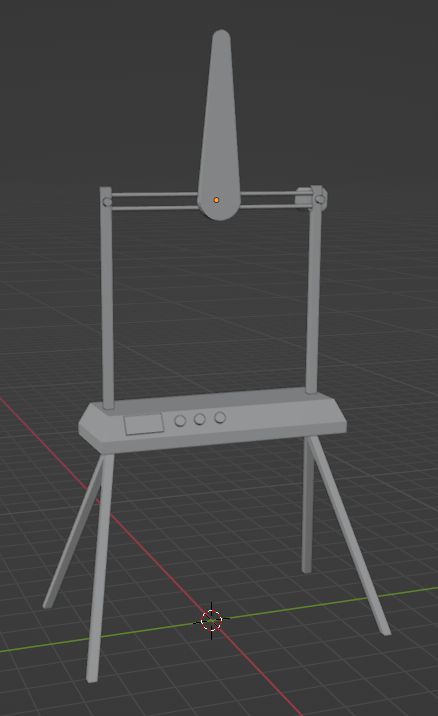
\includegraphics[height=7cm]{Full}
    \end{column}
\end{columns}

\end{frame}


\begin{frame}
\frametitle{Initial Renders (2/2)}

\begin{columns}
    \begin{column}{0.48\textwidth}
        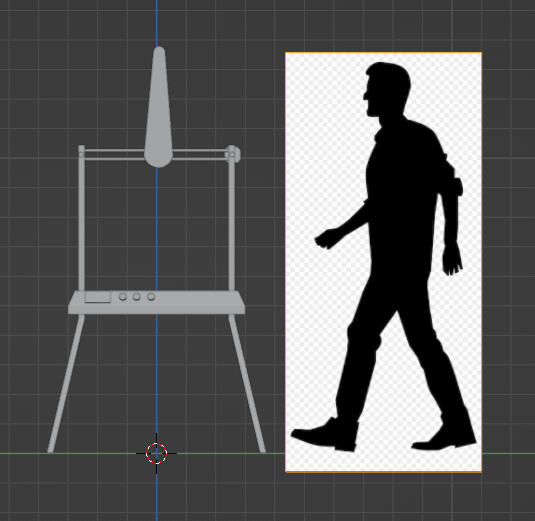
\includegraphics[width=5cm]{Scale}
    \end{column}
    \begin{column}{0.48\textwidth}
        \begin{block}{Initial Sketch}
            We'd like it to stand about this tall (left) to facilitate easy access
            and usage. With a simple and minimalist visible drivetrain (Below).
        \end{block}
        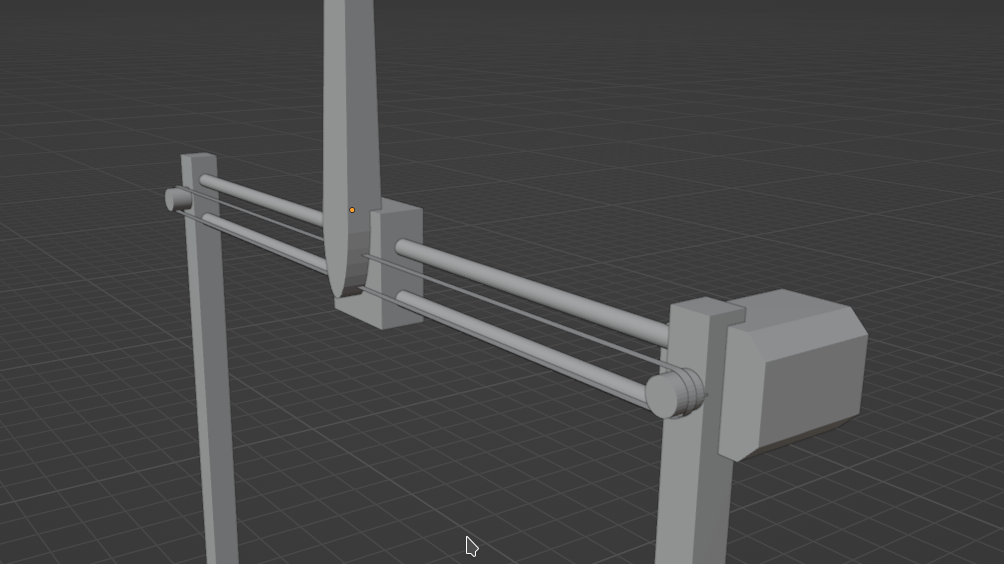
\includegraphics[width=5cm]{UpperAssy}
    \end{column}
\end{columns}

\end{frame}


\begin{frame}
\frametitle{End}

\begin{block}{}
    \begin{center}
        \Huge Questions and Comments?
    \end{center}
\end{block}

\begin{center}
    Find the source code for this document, and the rest of our designs, firmware, hardware
    and notes on GitHub!

    
\includegraphics[height=2cm]{github_qr}
\end{center}

\end{frame}


\end{document}
